\documentclass[12pt,a4paper,twoside]{article}
\usepackage{fancyhdr,graphicx,latexsym}

\setlength{\parindent}{0cm}
\setlength{\parskip}{2ex plus1ex minus 0.5ex}

\addtolength{\evensidemargin}{-2.5cm}
\addtolength{\oddsidemargin}{-0.5cm}
\addtolength{\textwidth}{3cm}

\addtolength{\headheight}{0.2cm}
\addtolength{\topmargin}{-1cm}
\addtolength{\textheight}{2.5cm}

\renewcommand{\_}{\texttt{\symbol{95}}}
\addtolength{\fboxsep}{0.1cm}
\newcommand{\param}[1]{\textit{\textrm{\textmd{#1}}}}
\newcommand{\codebar}{\rule{\textwidth}{0.3mm}}
% \newcommand{\spc}{\hspace{0.5mm}$\sqcup$\hspace{0.6mm}}
\newcommand{\spc}{\hspace{0.5mm}$\Box$\hspace{0.5mm}}
\newcommand{\todo}[1]{\textbf{TODO: #1}}

\newlength{\codelen}
\newcommand{\code}[1]
{\begin{center}\fbox{\parbox{16cm}{\texttt{#1}}}\end{center}}

\fancyhead{}
\fancyhead[RO,LE]{\thepage}
\fancyhead[LO,RE]{PIRATES User Guide}
\fancyfoot{}
\pagestyle{empty}

\newenvironment{bulletlist}
{
	\begin{itemize}
	\setlength{\itemsep}{0ex}
	\setlength{\parsep}{0ex}
}
{
	\end{itemize}
}

\newenvironment{alphalist}
{
	\begin{enumerate}
	\setlength{\itemsep}{0ex}
	\setlength{\parsep}{0ex}
	\renewcommand{\labelenumi}{(\alph{enumi})}
}
{
	\end{enumerate}
}

\newenvironment{numericlist}
{
	\begin{enumerate}
	\setlength{\itemsep}{0ex}
	\setlength{\parsep}{0ex}
}
{
	\end{enumerate}
}

\begin{document}

% \sfseries
\centerline{\textbf{\LARGE PIRATES User Guide}}
\begin{center} \large
David Ingram\\
TIME-EACM Project\\
University of Cambridge Computer Lab\\
13th August 2009\\
\end{center}

{ \parskip 0.1mm plus 0.1mm \tableofcontents }
\pagestyle{fancy}
% \newpage

\section{Requirements}

PIRATES is developed on Linux, although it should run on any POSIX
system without too much trouble. To build it gcc and GNU make
are recommended.

\section{Installation}

Run these commands to perform the installation (replace \verb^VER^ with
the appropriate version of the tarfile):

\begin{verbatim}
tar xzvf sbus_VER.tar.gz
cd sbus_VER
make -f Makefile.orig
make install
\end{verbatim}

The installation step will prompt for the directory prefix to install
to. You can install PIRATES as root or as a normal user.
If you run \verb^make install^ as root, the default installation prefix
suggested will be \verb^/usr/local^.
If you go with the default (recommended), this will install PIRATES into
\verb^/usr/local/bin^, \verb^/usr/local/lib^, \verb^/usr/local/include/sbus^,
\verb^/usr/local/doc/sbus^ and \verb^/usr/local/share/litmus^.
Note that \verb^/usr/local/bin^ must be in your \verb^$PATH^.

If \verb^make install^ is run instead as a normal user, the default prefix
suggested will be \verb^$HOME^. This environment variable must contain
the pathname of your home directory. Assuming you accept the default
location, binaries will then be installed to
\verb^$HOME/bin^, the library to \verb^$HOME/lib^, header files to
\verb^$HOME/include/sbus^, documentation to \verb^$HOME/doc/sbus^ and
metadata to \verb^$HOME/share/litmus^.
All of these directories will be created for you if they don't
already exist.
The binaries directory must be in your path. If it isn't, add the
following to your shell startup script (\verb^.bashrc^, for example):\\
\verb^export PATH=$PATH:$HOME/bin^

\subsection{Configuration}

\subsubsection*{a) \texttt{LITMUS\_PATH}}

At runtime, PIRATES needs to find metadata files and the master schemas.
It does this by consulting an environment variable called
\verb^$LITMUS_PATH^. This consists of a comma-separated list of
directories to look in for the files it needs. You can set the
environment variable to include any directories you use for
storing the metadata files.

The following directories are automatically appended to
\verb^$LITMUS_PATH^:\\
\verb^.,$HOME/share/litmus,/usr/local/share/litmus^\\
Also if the environment variable is not set at all, these
three directories are used.
Hence by default PIRATES will search the current directory, and the
default locations for the preinstalled schemas in both root
and non-root installations.

\subsubsection*{b) \texttt{SBUS\_INTERFACE}}

If you are running on a host which has more than one network interface
(not including loopback), you should set the \verb^$SBUS_INTERFACE^
environment variable. This specifies the interface whose IP address
will be used to uniquely identify the host (so the RDC can tell
when other components are running on the same machine, for example).

It is also concatenated with the port number each component is listening
on to form the canonical address for contacting that component, which
must be provided in certain circumstances. Consequently, if a host
with multiple network interfaces is connected to several otherwise
unconnected networks (i.e. not just several NICs connected to the
Internet) it is limited to interacting with PIRATES components on only one of
these networks, selected by the \verb^$SBUS_INTERFACE^ variable.

\section{Starting the resource discovery component}

One or more resource discovery components (RDCs) should be started before
launching any other components. PIRATES does not proscribe where you
run RDCs - you can run without one on a particular machine,
using a remote RDC instead, or you can run more than one RDC on
the same machine (although in the latter case they cannot all
listen to the default port, obviously). You can also use PIRATES as the
communications layer for P2P overlay networks, in which case you won't
run any RDCs at all since they will be replaced by your own
location service/algorithm.

Nevertheless the recommended approach in most cases will be to run exactly
one RDC on each machine which will host PIRATES components.
Indeed the RDC is capable of launching other PIRATES programs
(\textit{persistent components}) automatically, so when this feature is
used it may be the only process you really need to start.

Rather than starting the RDC manually, if you need reliable continuous
operation you should invoke it in system start up scripts instead, so
that it will restart if the machine is rebooted. An even better
approach is to also make cron try to restart it every five minutes or so.
This will ensure the system restarts in case the RDC crashes or is
killed for some reason. It is harmless to try and start the RDC when
one is already running on the same port; the second copy will
immediately exit.

The following command will run the RDC in the background (note: errors won't be
reported) at the default port:

\verb^rdc -bg^

Components do not need a RDC in order to function, however without
one you will need to identify them by their IP address and port number
which is much less convenient and flexible.

Synopsis:\\
\verb^rdc [ <option> ... ]^\\
\hspace*{15mm}\verb^-bg^ = run in background\\
\hspace*{15mm}\verb^-p <port>^ = specify port number\\
\hspace*{15mm}\verb^-a^ = use any port\\
\hspace*{15mm}\verb^-j <addr>^ = join (replicate) another RDC\\
\hspace*{15mm}\verb^-f <file>^ = join to multiple RDCs\\

If started without the \verb^-p^ or \verb^-a^ options, the new RDC
will try to bind to its default port (50123). It will abort if this
is not available (similarly in the case of \verb^-p^ if the port
requested is already in use).

\subsection{Replicated RDCs}

The RDC is not on any component's data path, and hence the system can
run for some time without it. It is however important for setting up
new connections, and is consequently a single point of failure. The
machine on which it is running may well be rebooted like any other, hence
for reliability it is a good idea to replicate the RDC.
RDCs never migrate, but additional replicas can be started and stopped.

Joining with other RDCs allows them to share information and
hence provide redundancy if one or more of them are killed.
A group of RDCs attempt to mirror the information received by any of
them as closely as possible.
The join option can be used more than once, to join with several
other RDCs.
The \verb^-f^ option refers to
a file, which should be in the format of one RDC address per line.
It is not an error if any of the RDCs specified
to join with are not running
(so it is safe to specify a file of many RDCs, some of which \textit{might}
be running).

Note that RDC addresses are always in one of the following forms:
\verb^dns.name^, \verb^dns.name:port^, \verb^n.n.n.n^
or \verb^n.n.n.n:port^. You cannot
use map constraints strings since RDCs do not register and hence
their locations cannot be looked up in other RDCs. If the port
number is omitted then the default RDC port (50123) is assumed.

\subsection{Specifying which RDCs components should use}

When you instantiate a component, a list is formed of RDCs
to try contacting. The list is a concatenation of:
\begin{bulletlist}
\item An environment variable: \verb^$SBUS_RDC_PATH^\\
      This should be formatted as a comma-separated list of addresses.
\item Any RDCs explicitly added by the application with the
      \verb^add_rdc()^ API call.\\
		Note: you may want to avoid this as it could hard-code addresses
		into your program.
\item The default port number at the local host.
\end{bulletlist}

The component will use all these RDCs for looking up other components, in
parallel. It will also register itself with all of these except for those
addresses which start with an exclaimation mark `!'. This is a special flag
which marks that address as lookup-only (useful for ``foreign'' RDCs
in other administrative domains).

It is safe to include RDC addresses where no RDC is running at the
time (possible locations). Caveat: currently this does introduce a
delay to component startup, whilst the attempt to connect times out
(this will be avoided in future). The intention is that it should also
be safe to register with multiple RDCs which happen to be federated,
although currently this may lead to duplicate registrations.

\section{Running the demo component}

The programs \verb^democpt^ and \verb^democlient^ illustrate
use of the library via a complete component and client.
Metadata for these components are in \verb^idl/demo.cpt^
and \verb^idl/democlient.cpt^.
The component implements five endpoints, to illustrate various
different access types.

You can run the demo component and client in any directory.
Make sure a compiled copy of the wrapper process called \verb^sbuswrapper^ is
placed somewhere in your path (the installation process does this for you).

\subsection{\texttt{democpt}}

Start the component with
\verb^democpt^. It will display the port number it is listening on.

\subsection{\texttt{democlient}}

Next, in another shell, run
\verb^democlient :portnum^, replacing \verb^portnum^ with the number
displayed by \verb^democpt^. The client will connect (map) to
the component and send some test messages and RPCs.

You can also try running \verb^speek -m :portnum^ and
\verb^speek -s :portnum^ to interrogate the demo component.

\subsection{Component addresses}

Other components to be mapped onto must be identified by a component
address. This is just a string which may contain any of the following
elements:

\begin{verbatim}
host:
:port
host:port
+Ncptname
+Iinstance
+Kkeyword
+Ucreator
+Ppeer
\end{verbatim}

% +Aancestor
% +S[endpoint][=<hash>[,<hash>]]
% +C[endpoint][=<hash>[,<hash>]]

% +Xkey

% +Ncptname Ccptname C=cptname cpt=cptname component=component
% +Iinstance I=instance inst=instance instance=instance
% +Kkeyword K=keyword word=keyword
% +Ucreator U=creator creator=creator
% +Xkey X=key pubkey=key
% +Ppeer P=peer peer=peer

% + comma or space

The first three elements are for direct addressing. The RDC is not
consulted if no other elements appear. Any of the others will
cause a RDC lookup in order to
locate components which meet the requirements. All of the elements
you specify must be satisfied (they are joined with an implicit
\textit{and}).
For example, \verb^+Nfoo+Pbar^ selects all \verb^foo^ components
which are connected to a \verb^bar^.
In addition, the hashcodes of the endpoint you are
mapping are added to the list of requirements automatically to
ensure a type-compatible match.

The \verb^P^ constraint specifies the names of other (peer) components
which must be connected to the component in question (or to be precise,
were connected at the time the RDC last pinged it for status information).
This allows you to
specify a component which is using a particular data supplier, for example.
\verb^peer^ may be a component or instance name.
Both the peer and keyword constraints may be specified more than once.

% The \verb^+S^ and \verb^+C^ elements are
% not currently used, because the hashcodes of the endpoint you are
% mapping are added to the list of requirements for you automatically.
% \verb^+S^ refers to sources and servers, whereas \verb^+C^ describes
% clients and sinks.

\section{Getting information}

\subsection{\texttt{speek}}

\verb^speek^ queries a component at a specified address for
its metadata and/or status information.

Synopsis:\\
\verb^speek (-m | -s | -e | -c) <address>^\\
\verb^speek schema <address> <endpoint>^\\
\verb^speek builtin <endpoint>^\\
\verb^speek builtins^\\
\hspace*{15mm}\verb^-m^ = metadata\\
\hspace*{15mm}\verb^-s^ = status\\
\hspace*{15mm}\verb^-e^ = endpoint info\\
\hspace*{15mm}\verb^-c^ = connection info\\

The \verb^-m^ and \verb^-s^ options dump large structures containing the
static metadata and dynamic status of the component, respectively.

The \verb^-e^ option prints a much more concise table of the
most useful information. The table lists the endpoints provided
by the component, and for each one displays their type, the
current number of peers they are mapped to, the number of
messages they have processed so far and whether a subscription
is in place.

A list of the peers each endpoint is connected to, together with all
subscriptions and topics, can be viewed with \verb^speek -c <address>^.

The \verb^schema^ option displays the message (and reply, if applicable)
schemas for a named endpoint; this is a subset of the information
returned by \verb^-m^. The \verb^builtin^ option does the same for a
named built-in endpoint, and \verb^builtins^ simply lists all
supported built-ins.

\subsection{\texttt{sbus}}

\verb^sbus^ queries the resource discovery component for information
about the currently registered components.

Synopsis:\\
\verb^sbus [-r <address>] list^ -- list summary information for all components\\
\verb^sbus [-r <address>] dump^ -- show all known information on all components (verbose)\\
\verb^sbus [-r <address>] links^ -- lists, for each component, which others they are
connected to\\
\verb^sbus [-r <address>] hup^ -- re-read persistent component list\\
\verb^sbus [-r <address>] start <command> <args...>^ -- remote start\\

The \verb^-r^ option specifies which RDC to ask. If omitted then the
default port on the localhost is assumed.

\subsection{\texttt{universalsink}}

\verb^universalsink^ is a component with a polymorphic sink endpoint,
which can be used to listen to and dump the contents of any stream
output by another component. The arguments specify the stream
source to connect to and an optional subscription for filtering
(at source).

Synopsis:\\
\verb^universalsink [Options] <address> <endpoint> [<instance-name>]^\\
\verb^universalsink [-x] -u [<instance-name>]^\\
\verb^Options: -t <topic>^\\
\verb^         -s <subscription>^\\
\verb^         -x^\\

The \verb^-u^ flag instructs \verb^universalsink^ to start unmapped.
In either case, any messages received are output to stdout
as plain text, or as XML if the \verb^-x^ flag is specified.

\subsection{\texttt{universalsource}}

Synopsis:\\
\verb^universalsource <schema-file> [<instance-name>]^\\

This component provides a single source endpoint, of type corresponding
to the schema contained in \verb^schema-file^. Messages in XML are
read from stdin and output on this endpoint. Each message must be
separated by a blank line.

\section{Reconfiguring running components}

\subsection{\texttt{spoke}}

\verb^spoke^ can be used to map and unmap pairs of component endpoints.

Synopsis:\\
\verb^spoke map    <address> <endpoint> <to addr> <to endpt>^\\
\verb^spoke unmap  <address> <endpoint>^\\
\verb^spoke divert <address> <endpoint> <new addr> <new endpt>^\\
\verb^spoke subscribe <addr> <endpoint> <subs-expr> [<peer-cpt> | '*']^\\
\verb^spoke topic  <address> <endpoint> <topic>     [<peer-cpt> | '*']^\\
\verb^spoke emit   <address> <endpoint> <schema-file> [<XML>]^\\
\verb^spoke rpc    <address> <endpoint> <schema-file> <schema-file> [<XML>]^\\
\verb^spoke send   <address> <endpoint> [<XML>]^\\
\verb^spoke log    <address> <log-level> <echo-level>^\\
\verb^spoke terminate <address>^\\

The \verb^divert^ option causes all peer components which are
connected to the given address and endpoint to disconnect and
remap to the new location.

When using \verb^subscribe^ or \verb^topic^
you have the option of changing the subscription for one
currently mapped peer (specified by component or instance name),
for all currently mapped peers (specified by \verb^'*'^), or to
set the default subscription for all future maps (by omitting
the final argument).

Log levels are formed by summing the following: 1 = errors,
2 = warnings, 4 = messages, 8 = debug.

The \verb^emit^, \verb^rpc^ and \verb^send^ options can be used as
a universal client to send messages to any component. The message
is expressed in XML, either in a string as the final argument, or
if omitted then read from stdin instead (type in your message and
press CTRL-d for end-of-file when done). The first two use files
to specify the schemas for the message being sent, and reply
for RPCs. The \verb^send^ option instead interrogates the target
component first to discover what schemas it uses.

\section{Persistent components}

If you have components you would like to always run on a particular
machine, and if you have arranged for a RDC to be automatically started
there first, you may declare \textit{persistent components} which it
will ensure run at all times.

Persistent components are automatically launched
\begin{numericlist}
\item [a)] when the RDC starts
\item [b)] when an existing persistent component deregisters
\item [c)] when a component fails to respond to a periodic ping\\[1mm]
	and indirectly (since this causes a ping):
\item [d)] when the RDC receives a ``lost'' event for them from
	a third party component, indicating they have lost contact with
	the persistent component.
\end{numericlist}

This list of persistent components is read from the file
\verb^$SBUS_DIR/autorun^ (or \verb^~/.sbus/autorun^ if
\verb^$SBUS_DIR^ is not set).
The RDC checks which components are already running by consulting
the \verb^/proc^ filesystem. Components must be invoked with exactly
the same pathname and arguments as those given in the autorun file
so that they are recognised as the same thing.
Components are started with \verb^fork^ and \verb^exec^, and hence
run as the same user and group as the RDC.

%\section{Persistent links}
%
%Not implemented yet!
%
%\section{Example}
%
%TODO

\section{Running an event broker}
\label{broker}

Synopsis:\\
\verb^broker [-bg] [port-num]^\\
\hspace*{15mm}\verb^-bg^ = run in background\\

This is a general-purpose event broker.
It has one sink endpoint which
accepts any message, and one source which outputs everything
received. The wrapper's built-in subscription matching takes care of
the rest; content and topic based subscriptions are therefore provided.
This component is polymorphic, because its endpoints handle
messages of any type (specfied by the \verb^"*"^ schema).

% \begin{figure}[htbp]
\begin{figure}[ht]
\centering
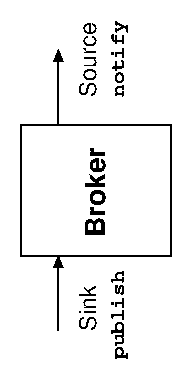
\includegraphics[scale=1.0,angle=-90]{diagrams/broker.eps}
% \caption{Communication types}
% \label{broker}
\end{figure}

\section{Creating your own component}

\subsection{Writing schemas}

\textbf{\texttt{\large $\bullet$ checkschema}}

Synopsis:
\verb^checkschema [-v] [-q] schema-file ...^

This utility parses a schema and reports any errors.

\textbf{\texttt{\large $\bullet$ litmuscode}}

Synopsis:
\verb^litmuscode <filename>^

Given a file containing a schema (and nothing
else), this program calculates the schema's LITMUS code for you.
It outputs it as a 12 digit hexadecimal number. You can use this value
in your programs which will implement endpoints with this schema in order
for the type checking to work. \verb^filename^ may be \verb^-^ to
read from \verb^stdin^.

\subsection{Creating metadata}

You must create a file containing the standard metadata for your
component before you can instantiate it. Give this file the
\verb^.cpt^ extension and place it in one of the directories
searched for metadata (see the Configuration section above).

The easiest method is to copy and then edit an existing metadata file,
for example\\
\verb^cp demo.cpt foo.cpt^\\
Change the administrative fields and then add or delete endpoint
sections based on the number your component needs 
(both for services provided, and those accessed as a client).
Then fill in the endpoint names, types and schemas.

Run \verb^analysecpt foo.cpt^ to test parsing of your new metadata file.

\textbf{\texttt{\large $\bullet$ checkmetadata}}

Synopsis:
\verb^checkmetadata <component-metadata-file> ...^

Checks that a component metadata file complies
with the master schema.

\textbf{\texttt{\large $\bullet$ analysecpt}}

Synopsis:
\verb^analysecpt [-q] <component-metadata-file>^

The argument to this utility should be
a file containing a complete component's metadata (e.g. \verb^demo.cpt^).
It parses the file according to the master schema and extracts
the essential information about the names and types of the endpoints.
It also calculates
the LITMUS codes for all the schemas it finds, which is quicker
to use than pasting each schema individually into \verb^litmuscode^.
The \verb^-q^ option omits the schema text, in order to display a
more compact summary.

\subsection{Writing code}

Check the demo source code for examples of typical use of the API.
\verb^democlient.cpp^ illustrates sequential invocation of library
routines, and \verb^democpt.cpp^ shows an event loop which waits for
activity from the library. The demo component uses the \verb^multiplex^
utility object, which wraps \verb^select()^ in a simpler API, but you
can of course use \verb^select()^ directly instead, if you prefer.

\subsection{Compiling}

Make sure the source code for your component includes the line\\
\verb^#include <sbus/sbus.h>^

Then, if PIRATES was installed as root, build your component with a Makefile
like this:
\begin{verbatim}
foo: foo.cpp
   g++ -o foo foo.cpp -lsbus
\end{verbatim}

If PIRATES has \textit{not} been installed as root,
use a Makefile like this instead:
\begin{verbatim}
foo: foo.cpp
   g++ -I ${HOME}/include -L ${HOME}/lib -o foo foo.cpp -lsbus
\end{verbatim}

\section{Storage utilities}

\subsection{\texttt{archive}}

\verb^archive^ -- this takes a schema, a file containing a batch
of messages encoded in the XML disk file format (described in the
protocol document), and an output archive filename. The XML file is
parsed and the messages within checked against the schema. They
are then converted to the binary archive format and written out to the
output file (which is overwritten if it already exists). The
\verb^archive^ tool is currently limited to files containing
messages which are all of the same type (this restriction will
be lifted in future).

\subsection{\texttt{extract}}

\verb^extract^ -- this is the opposite of \verb^archive^. You
must specify a schema and a binary archive file. After validation
the messages in the binary archive file are output in the XML
file format to the terminal. \verb^extract^ is also currently
limited to files containing messages of a single type only.

\end{document}
